%%%%%%%%%%%%%%%%%%%%%%%%%%%%%%%%%%%%%%%%%%%%%%%%%%%%%%%%%%%%%%%%%%%%%%%%%%%%%%%%%%%%%%%%%%%%%%%%%%%%%%
% Plantilla básica de Latex en Español.
%
% Autor: Andrés Herrera Poyatos (https://github.com/andreshp) 
%
% Es una plantilla básica para redactar documentos. Utiliza el paquete fancyhdr para darle un
% estilo moderno pero serio.
%
% La plantilla se encuentra adaptada al español.
%
%%%%%%%%%%%%%%%%%%%%%%%%%%%%%%%%%%%%%%%%%%%%%%%%%%%%%%%%%%%%%%%%%%%%%%%%%%%%%%%%%%%%%%%%%%%%%%%%%%%%%%

%-----------------------------------------------------------------------------------------------------
%	INCLUSIÓN DE PAQUETES BÁSICOS
%-----------------------------------------------------------------------------------------------------

\documentclass{article}


%-----------------------------------------------------------------------------------------------------
%	SELECCIÓN DEL LENGUAJE
%-----------------------------------------------------------------------------------------------------

% Paquetes para adaptar Látex al Español:
\usepackage[spanish,es-noquoting, es-tabla, es-lcroman]{babel} % Cambia 
\usepackage[utf8]{inputenc}                                    % Permite los acentos.
\selectlanguage{spanish}                                       % Selecciono como lenguaje el Español.

%-----------------------------------------------------------------------------------------------------
%	SELECCIÓN DE LA FUENTE
%-----------------------------------------------------------------------------------------------------

% Fuente utilizada.
\usepackage{courier}                    % Fuente Courier.
\usepackage{microtype}                  % Mejora la letra final de cara al lector.

%-----------------------------------------------------------------------------------------------------
%	IMÁGENES
%-----------------------------------------------------------------------------------------------------

\usepackage{float}

%-----------------------------------------------------------------------------------------------------
%	ESTILO DE PÁGINA
%-----------------------------------------------------------------------------------------------------

% Paquetes para el diseño de página:
\usepackage{fancyhdr}               % Utilizado para hacer títulos propios.
\usepackage{lastpage}               % Referencia a la última página. Utilizado para el pie de página.
\usepackage{extramarks}             % Marcas extras. Utilizado en pie de página y cabecera.
\usepackage[parfill]{parskip}       % Crea una nueva línea entre párrafos.
\usepackage{geometry}               % Asigna la "geometría" de las páginas.

% Se elige el estilo fancy y márgenes de 3 centímetros.
\pagestyle{fancy}
\geometry{left=3cm,right=3cm,top=3cm,bottom=3cm,headheight=1cm,headsep=0.5cm} % Márgenes y cabecera.
% Se limpia la cabecera y el pie de página para poder rehacerlos luego.
\fancyhf{}

% Espacios en el documento:
\linespread{1.1}                        % Espacio entre líneas.
\setlength\parindent{0pt}               % Selecciona la indentación para cada inicio de párrafo.

% Cabecera del documento. Se ajusta la línea de la cabecera.
\renewcommand\headrule{
	\begin{minipage}{1\textwidth}
	    \hrule width \hsize 
	\end{minipage}
}

% Texto de la cabecera:
\lhead{\subject}                          % Parte izquierda.
\chead{}                                    % Centro.
\rhead{\doctitle \ - \docsubtitle}              % Parte derecha.

% Pie de página del documento. Se ajusta la línea del pie de página.
\renewcommand\footrule{                                 
\begin{minipage}{1\textwidth}
    \hrule width \hsize   
\end{minipage}\par
}

\lfoot{}                                                 % Parte izquierda.
\cfoot{}                                                 % Centro.
\rfoot{Página\ \thepage\ de\ \protect\pageref{LastPage}} % Parte derecha.


%----------------------------------------------------------------------------------------
%   MATEMÁTICAS
%----------------------------------------------------------------------------------------

% Paquetes para matemáticas:                     
\usepackage{amsmath, amsthm, amssymb, amsfonts, amscd} % Teoremas, fuentes y símbolos.
     
 % Nuevo estilo para definiciones
 \newtheoremstyle{definition-style} % Nombre del estilo
 {5pt}                % Espacio por encima
 {0pt}                % Espacio por debajo
 {}                   % Fuente del cuerpo
 {}                   % Identación: vacío= sin identación, \parindent = identación del parráfo
 {\bf}                % Fuente para la cabecera
 {.}                  % Puntuación tras la cabecera
 {.5em}               % Espacio tras la cabecera: { } = espacio usal entre palabras, \newline = nueva línea
 {}                   % Especificación de la cabecera (si se deja vaía implica 'normal')
 
 % Nuevo estilo para teoremas
 \newtheoremstyle{theorem-style} % Nombre del estilo
 {5pt}                % Espacio por encima
 {0pt}                % Espacio por debajo
 {\itshape}           % Fuente del cuerpo
 {}                   % Identación: vacío= sin identación, \parindent = identación del parráfo
 {\bf}                % Fuente para la cabecera
 {.}                  % Puntuación tras la cabecera
 {.5em}               % Espacio tras la cabecera: { } = espacio usal entre palabras, \newline = nueva línea
 {}                   % Especificación de la cabecera (si se deja vaía implica 'normal')
 
 % Nuevo estilo para ejemplos y ejercicios
 \newtheoremstyle{example-style} % Nombre del estilo
 {5pt}                % Espacio por encima
 {0pt}                % Espacio por debajo
 {}                   % Fuente del cuerpo
 {}                   % Identación: vacío= sin identación, \parindent = identación del parráfo
 {\scshape}                % Fuente para la cabecera
 {:}                  % Puntuación tras la cabecera
 {.5em}               % Espacio tras la cabecera: { } = espacio usal entre palabras, \newline = nueva línea
 {}                   % Especificación de la cabecera (si se deja vaía implica 'normal')
 
 % Teoremas:
 \theoremstyle{theorem-style}  % Otras posibilidades: plain (por defecto), definition, remark
 \newtheorem{theorem}{Teorema}[section]  % [section] indica que el contador se reinicia cada sección
 \newtheorem{corollary}[theorem]{Corolario} % [theorem] indica que comparte el contador con theorem
 \newtheorem{lemma}[theorem]{Lema}
 \newtheorem{proposition}[theorem]{Proposición}
 
 % Definiciones, notas, conjeturas
 \theoremstyle{definition-style}
 \newtheorem{definition}{Definición}[section]
 \newtheorem{conjecture}{Conjetura}[section]
 \newtheorem*{note}{Nota} % * indica que no tiene contador
 
 % Ejemplos, ejercicios
 \theoremstyle{example-style}
 \newtheorem{example}{Ejemplo}[section]
 \newtheorem{exercise}{Ejercicio}[section]

%-----------------------------------------------------------------------------------------------------
%	BIBLIOGRAFÍA
%-----------------------------------------------------------------------------------------------------

\usepackage[backend=bibtex, style=numeric]{biblatex}
\usepackage{csquotes}

\addbibresource{references.bib}

%-----------------------------------------------------------------------------------------------------
%	PORTADA
%-----------------------------------------------------------------------------------------------------

% Elija uno de los siguientes formatos.
% No olvide incluir los archivos .sty asociados en el directorio del documento.
\usepackage{title1}
%\usepackage{title2}
%\usepackage{title3}

%-----------------------------------------------------------------------------------------------------
%	TÍTULO, AUTOR Y OTROS DATOS DEL DOCUMENTO
%-----------------------------------------------------------------------------------------------------

% Título del documento.
\newcommand{\doctitle}{Ecuaciones diferenciales ordinarias}
% Subtítulo.
\newcommand{\docsubtitle}{Método del trapecio}
% Fecha.
\newcommand{\docdate}{1 \ de \ Enero \ de \ 2015}
% Asignatura.
\newcommand{\subject}{Métodos Numéricos II}
% Autor.
\newcommand{\docauthor}{Andrés Herrera Poyatos \\ Javier Poyatos Amador \\ Rodrigo Raya Castellano}
\newcommand{\docaddress}{Universidad de Granada}
\newcommand{\docemail}{}

%-----------------------------------------------------------------------------------------------------
%	RESUMEN
%-------------------------------					----------------------------------------------------------------------

% Resumen del documento. Va en la portada.
% Puedes también dejarlo vacío, en cuyo caso no aparece en la portada.
%\newcommand{\docabstract}{}
\newcommand{\docabstract}{En este texto puedes incluir un resumen del documento. Este informa al lector sobre el contenido del texto, indicando el objetivo del mismo y qué se puede aprender de él.}

\begin{document}

\maketitle

%-----------------------------------------------------------------------------------------------------
%	ÍNDICE
%-----------------------------------------------------------------------------------------------------

% Profundidad del Índice:
%\setcounter{tocdepth}{1}

\newpage
\tableofcontents
\newpage

%-----------------------------------------------------------------------------------------------------
%	SECCIÓN 1: MOTIVACIÓN
%-----------------------------------------------------------------------------------------------------

\section{Motivación: ecuaciones diferenciales ordinarias de primer orden} \label{sec:motivacion}

	\begin{definition} 
		Dada una función $f:\Omega \subseteq \mathbb R^2  \to \mathbb{R}$ continua, una un problema de valores iniciales de primer orden consiste en encontrar aquellas funciones $y: [a,b] \rightarrow \mathbb{R}$ de clase 1 que verifiquen $G(y) \subset \Omega$, $y'(t) = f(t,y(t)) \ \forall t \in [a,b]$ y la condición inicial $y(t_0) = y_0$, donde $t_0 \in [a,b]$.  
	\end{definition}

	De forma simplificada, un problema de valores iniciales se representa de la siguiente forma: 
	\begin{equation*}
		\begin{cases}
			y'(t) = f(t,y(t)) \\
			y(t_0) = y_0 \\
			t \in [a,b]
		\end{cases}
	\end{equation*}

	Resolver de forma exacta un problema de valores iniciales es muy difícil. Existen ecuaciones diferenciales como $y'(t)^2 + y(t)^2 + 1 = 0$ de las cuales no se conoce una solución exacta. Sin embargo, existen múltiples resultados que permiten asegurar la existencia y unicidad de soluciones de la ecuación diferencial incluso cuando no se puedan obtener soluciones explícitamente.

	Uno de los objetivos de la teoría del Análisis Numérico en el campo de las ecuaciones diferenciales ordinarias es resolver de forma aproximada problemas de valores iniciales una vez se conoce la existencia y unicidad de soluciones. Para ello, una técnica habitual son los métodos de discretización que son cualquier método numérico que trata obtener valores aproximados de una sucesión $y_n$ de la solución $y(x)$ en los diferentes nodos $x_n$ que se obtienen al realizar la partición del intervalo en el que se trabaja. Se toman $n+1$ puntos $t_0, t_1, \ldots, t_n \in [a.b]$ con $a = t_0 < t_1 < \ldots < t_n = b$ y se intenta aproximar la imagen de la solución del problema de valores iniciales en estos puntos. Es habitual denotar a las aproximaciones obtenidas $w_i$. En lo que sigue, se trabajará siempre con condiciones iniciales sobre $y(a)$ para simplificar la definición de los métodos de discretización. 	
	
	\textbf{Repasar estos dos párrafos, no sé si queda claro.}La primera idea intuitiva para resolver este problema consiste en interpretar la primera ecuación como un campo vectorial aprovechando la definición de derivada como aproximación lineal de la función en un punto. Esto es, $f$ le asigna a cada punto la dirección en la que varía cualquier solución del problema que pase por ese punto.

	\begin{figure}[h]
		\centering
		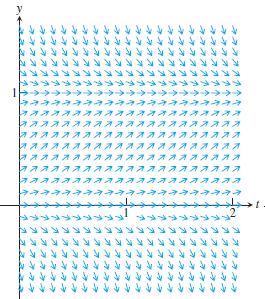
\includegraphics[width=4cm]{./Images/interpret-pvi.png}
		\caption{Representación del campo vectorial asociado a la ecuación logística $y'(t) = c y(t) (1 - y(t))$.} 
		\label{fig:interpret-pvi}
	\end{figure}

	Si conocemos la imagen de la solución $y$ en un punto $t_{i-1}$, entonces sabemos que en ese punto la función variará en la dirección dada por el campo vectorial comentado previamente. Nótese que esta es la dirección de la recta tangente a $y$ en $t_{i-1}$. Podemos utilizar la imagen de esta recta tangente en $t_{i+1}$ para aproximar $y(t_{i+1})$. Repitiendo el proceso para aproximar $y(t_{i+2})$ a partir de $w_{i+1}$, se obtiene el método de Euler cuya expresión resumida es la siguiente:

	\begin{center}
		$\begin{cases}
		w_0=y_0 \\
		h_{i} = t_{i+1} - t_i \\
		w_{i+1} = w_i + h_{i} f(t_i,w_i)
		\end{cases}$
	\end{center}
	
	Los mejores resultados se obtienen mediante el uso de puntos equidistantes, esto es, $h = \frac{b-a}{n}$ y $t_i = a + ih \ \forall i = 0 \ldots n$. En el resto del texto se trabajará siempre con puntos equidistantes. El estudio del método de Euler concluye que el error global de aproximación cometido es $O(h)$, esto es, existe $M \ge 0$ tal que $\left|y_i - w_i\right| \le\dfrac{Mh}{2}$ para todo $i=0 \ldots n$.
				
	A priori, puede parecer que el método de Euler es válido en cualquier aplicación simplemente reduciendo el valor de $h$, esto es, aproximando un mayor número de puntos. Sin embargo, a continuación estudiaremos un ejemplo para el cual el método de Euler requiere una excesiva cantidad de puntos para obtener un error de aproximación aceptable. 
	
	\textbf{EJEMPLO DEL MÉTODO DE EULER. MEJORAR}
	
	\begin{example} Considérese el siguiente problema de valores iniciales
		\begin{equation*}
			\begin{cases}
			y'(t) = -4 t^3 y^2 \\
			y(-10) = 1/10001 \\
			t \in [-10,0] \\
			\end{cases}
		\end{equation*}

		La solución exacta de este problema es $y(t)=\frac{1}{1+t^4}$. La Tabla \ref{table:euler} muestra los resultados de aproximación obtenidos por el método de Euler en $y(0)$ para distintos valores de $h$. Se observa que la aproximación obtenida deja mucho que desear a pesar de haber llegado a utilizar hasta un millón de puntos. 
	\end{example}
	
	\begin{table}[H]
		\centering
		\begin{tabular}{|| c | c | c ||}
			\hline
			\hline $N$ &  $h$ & $w_n$ \\
			\hline 100 & 0.1 & 0.00390138 \\
			\hline 1000 & 0.01 & 0.03085162 \\
			\hline 5000 & 0.002 & 0.13282140 \\
			\hline 7500 & 0.0013 & 0.18614311 \\
			\hline 10000 & 0.001 & 0.23325153 \\			
		\end{tabular}
		\caption{Ejemplo práctico del método de Euler.}
		\label{table:euler}
	\end{table}
	
	\begin{figure}[H]
		\centering
		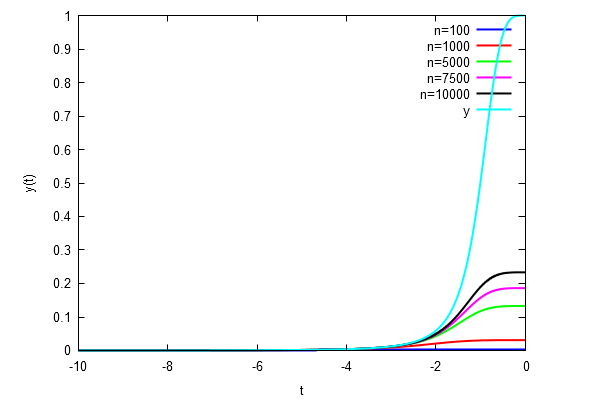
\includegraphics[width=0.7\textwidth]{./Images/eulermaxima.png}
		\label{fig:euler}
		\caption{Aproximaciones de $y(t)$ obtenidas con el método de Euler para diferentes valores de $n$.}
	\end{figure}
	
	El objetivo de este trabajo es introducir un método de discretización para aproximar soluciones de problemas de valores iniciales que presente menor error que el método de Euler. El método en cuestión se conoce como método del trapecio y presenta dos variantes denominadas explícita e iterativa. 
	
	El trabajo se organiza como sigue. En la Sección \ref{sec:previo} se explican algunas definiciones y resultados sobre la existencia, unicidad y estabilidad de las soluciones que serán necesarios posteriormente. En la Sección \ref{sec:intro-trapecio} se muestra la idea a partir de la cual surgen las diferentes versiones del método del trapecio. Posteriormente, en las Secciones \ref{sec:trapecio-explicito} y \ref{sec:trapecio-iterativo} se desarrollan los métodos del trapecio explícito e iterativo respectivamente. Ambos métodos se estudian desde una doble perspectiva: cálculo del error y estabilidad de las soluciones. Además, se muestra cómo los errores de redondeo afectan al comportamiento del método. En la Sección \ref{sec:paper} se resume el artículo de investigación "Nombre del artículo", que pone de manifiesto que la resolución de problemas de valores iniciales sigue siendo un tema abierto en la actualidad. Por último, en la Sección \ref{sec:conclusion} se destacan las conclusiones obtenidas y las ventajas y desventajas del método del trapecio.
	
\section{Definiciones y resultados previos.} \label{sec:previo}
	
	En esta sección se proporcionan las definiciones y resultados que se necesitan para el estudio del método del trapecio. En primer lugar, una de las hipótesis con las que se suele trabajar para problemas de valores iniciales es que la función $f$ sea lipschitziana en la segunda variable.
	
	\begin{definition}
		Sea $S = [a,b] \times [\alpha, \beta] \subseteq \mathbb R^2.$ Se dice que una función $f(t,y)$ es de Lipschitz respecto a la segunda variable, $y$, si existe una constante $L$, llamada constante de Lipschitz de forma que $|f(t,y_1) - f(t, y_2)| \le L * |y_1 - y_2|,  \forall (t,y_1), (t,y_2) \in S $.  
	\end{definition}
	
	No tiene sentido aplicar un método numérico para resolver un problema de valores iniciales que no tenga solución. Por tanto, los resultados que garanticen la existencia de soluciones al problema son fundamentales en este contexto. Además, si el problema admitiese varias soluciones distintas, entonces el método puede no comportarse correctamente pues no se sabe cuál debe calcular. Por tanto, la unicidad de soluciones también es un concepto que se debe estudiar en profundidad. El resultado de este estudio se resume en el teorema de existencia y unicidad de soluciones, que utiliza como hipótesis fundamental el concepto de función lipschitziana en la segunda variable.
	
	\begin{theorem} \label{theorem:existence-uniqueness}
		(Existencia y unicidad de soluciones) Sea $f: [a,b]\times[\alpha,\beta] \rightarrow \mathbb{R}$ e $y_0 \in (\alpha,\beta)$. Entonces:
		\begin{enumerate}
			\item Si f es Lipschitz en $[a,b]\times[\alpha,\beta]$, entonces existe $c \in [a,b]$ tal que el problema de valores iniciales:
			\begin{center}
				$\begin{cases}
				y'(t) = f(t,y(t)) \\
				y(a) = y_0 \\
				t \in [a,c] \\
				\end{cases}$
			\end{center}
			tiene exactamente una solución. 
			\item Si f es Lipschitz en $[a,b]\times]-\infty,\infty[$, entonces existe exactamente una solución en $[a,b]$	
		\end{enumerate}
	\end{theorem}
	
	\textbf{Demostración en caso de tener tiempo.}
 
	Nótese que el resultado es válido para cualquier condición inicial escogida. Esto es, la existencia y unicidad solamente depende de $f$. De aquí en adelante siempre se supondrá que el problema de valores iniciales a resolver tiene solución y que esta es única. En la práctica este hecho es algo que habrá que comprobar mediante el Teorema \ref{theorem:existence-uniqueness}. Bajo hipótesis de existencia y unicidad se pueden definir $y_i$ como los valores que toma la solución en los puntos $t_i = a + ih$ para todo $i = 0 \ldots n$, donde $h = \frac{b-a}{n}$ .
 
	El estudio de los métodos numéricos para problemas de valores iniciales se centra en la acotación de los errores cometidos y en el análisis de la estabilidad de los métodos. Las demostraciones de resultados asociados a estos conceptos suelen requerir el uso de múltiples desigualdades. El siguiente resultado, basado en la desigualdad de Gronwall, proporciona una de las desigualdades con más aplicaciones en esta área.
	
	\begin{theorem}
		Sean dos soluciones $y(t), z(t)$ de los problemas de valores iniciales con ecuación $y'(t) = f(t,y(t))$ y condiciones iniciales $y(a)$ y $z(a)$, respectivamente. Supóngase que f es de Lispchtiz en $[a,b]\times[\alpha,\beta]$. Entonces $|y(t)-z(t)| \leq e^{L(t-a)}|y(a)-z(a)|$ donde L es la constante de Lipschitz de f.
	\end{theorem}

	Un método será mejor que otro cuanto menor error presenten las aproximaciones obtenidas. Sin embargo, el concepto de error se puede ampliar introduciendo los errores locales y globales.
	
	\begin{definition} 
		Sean $w_i$ los valores estimados en los puntos $t_i$ por cierto método de aproximación. Sea también $z_i$ el valor de la solución exacta en $t_i$ para el problema de valores iniciales
		
		\begin{center}
			$\begin{cases}
			y'(t) = f(t,y(t)) \\
			y(t_{i-1}) = w_{i-1} \\
			t \in [t_{i-1},t_{i}] \\
			\end{cases}$
		\end{center}

		Se definen los siguientes errores:
	
		\begin{itemize}
			\item Error global de truncatura o error acumulado en el nodo i-ésimo: $g_i=|y_i - w_i|$
			\item Error local de truncatura o error en un paso: $e_i = |z_i - w_i|$
		\end{itemize} 
	\end{definition}
	
	Dicho de otro modo, el error local es el error cometido al avanzar la solución desde $t_{j-1}$ hasta $t_j$ suponiendo que $y_{j-1}$ que $y_{j-1}$ es exacto. Se trata del error que se comete al aproximar $\int_{t_{j-1}}^{t_{j}} f(t,y(t)) dt$. 
	Por otro lado, el error global tiene en cuenta que los errores cometidos en los $j-1$ pasos anteriores pueden haberse acumulado en $y_{j-1}$. Si a este error le añadimos el error local cometido en el paso $j$ obtenemos el error global de $y_j$.
	Por tanto, el error global cometido en cualquier paso puede entenderse por la suma del error local y el error global del paso previo amplificado. Este hecho se puede visualizar en la Figura \ref{fig:error}, que ejemplifica los conceptos de errores locales y globales.
		
	\begin{figure}[h]
		\centering
		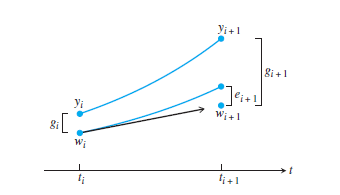
\includegraphics[width=10cm]{./Images/error-euler.png}
		\caption{Representación gráfica de los errores locales y globales.} 
		\label{fig:error}
	\end{figure}
	
	La relación entre errores locales y errores globales viene dada por el siguiente teorema: \\
	
	\begin{theorem} \label{theorem:local-global-error}
		Supóngase que la función $f$ es lipschitziana en la segunda variable con constante de Lipschitz $L$. Además, supóngase que existen $C \ge 0$ y $k \in \mathbb{N}$ tales que los errores locales verifican $e_i \le C h^{k+1}$ para todo $i = 0 \ldots n$. Entonces, se verifica la siguiente desigualdad para los errores globales
		\begin{equation}
			g_i \le \frac{C h^k}{L} (e^{L(t_i-a)}-1)
		\end{equation}
	\end{theorem} 
	\begin{proof}
		En breve.
	\end{proof}
	
	La siguiente definición pone nombre a las acotaciones del Teorema \ref{theorem:local-global-error}.
	
	\begin{definition} 
		Considérese un método de discretización para problemas de valores iniciales. Entonces:
		\begin{enumerate}
			\item El método es localmente de orden $k$ si existe una constante $C \ge 0$ tal que $e_i \le C h^k$ para todo $i = 0 \ldots n$.
			\item El método es de orden $k$ si existe una constante $C \ge 0$ tal que $g_i \le C h^k$ para todo $i = 0 \ldots n$.
		\end{enumerate}
	\end{definition}
	
	Las constantes de la definición previa dependerán del problema de valores iniciales en cuestión. Nótese que el Teorema \ref{theorem:local-global-error} está diciendo si un método es localmente de orden $k+1$, entonces es de orden $k$. Como aplicación directa de este teorema se obtiene fácilmente el orden del método de Euler.
	
	\begin{theorem}
		Supóngase que $f: [a,b] \times ]-\infty, +\infty[ \rightarrow \mathbb{R}$ es derivable y lipschitziana en la segunda variable. Entonces, el método de Euler es localmente de orden $2$. Consecuentemente, el método de Euler es de orden $1$.
	\end{theorem}
	
	\begin{proof}
		Sea $y$ la solución del problema de valores iniciales para $y(a) = y_0$. Fijemos $i = 1 \ldots n$ y sea $z$ la solución del problema de valores iniciales para $z(t_{i-1}) = w_{i-1}$. Por inducción, $z$ es de clase infinito. El teorema de Taylor para orden 2 proporciona la siguiente igualdad para cualquier 
		\begin{equation}
			z_i= w_{i-1} + h f(t_{i-1}, w_{i-1}) + \frac{h^2}{2} z''(\xi_i) = w_i + \frac{h^2}{2} z''(\xi_i)
		\end{equation}

		donde $\xi_i \in [t_{i-1}, t_i]$. Por tanto, si se utiliza esta igualdad en la expresión del error local se tiene
		\begin{equation}
			e_i = |z_i - w_i| = \left|\frac{h^2}{2} z''(\xi_i)\right| \le \frac{M_i}{2} h^2
		\end{equation}

		donde $M_i = \max\{z''(t) : t \in [t_{i-1}, t_i]\}$. Tomando $M = \max_{i = 1 \ldots n} M_i$, se tiene que el método de Euler es localmente de orden 2 como se quería. La prueba la cierra la aplicación del Teorema \ref{theorem:local-global-error}.
	\end{proof}
	
	En general, un método de un paso para aproximar la solución de una ecuación diferencial es un método que puede ser escrito de la forma $y_{i+1}=y_i + h \phi(t_i,y_i,h)$ donde $\phi$ es una función de $f, t_i, y_i$ y $h$. 
	
	\begin{definition}
		\textbf{Creo que está mal.} Diremos que el método de un paso anterior es convergente si:
		\begin{enumerate}
			\item $y_n \to y(t)$ para todo $0 \le t \le b$ según $n \to \infty$ y 
			\item $y_0 \to y(0)$ con $h=t/n$
		\end{enumerate}
		para cualquier ecuación diferencial $y'=f(y)$ que satisfaga una condición de Lipschitz.
	\end{definition}
	
	Por tanto, si el orden del método es $O(h^r)$ con $r > 0$, se tiene que el método es convergente.
	
	\begin{definition}
		Diremos que el método de un paso anterior es estable si para cada ecuación diferencial que satisfaga una condición de Lipschit existen constantes positivas $h_0$ y $K$ tales que la diferencia entre dos soluciones obtenidas numéricamente $y_n$ e $w_n$ es tal que $||y_n-w_n|| \leq K ||y_o-w_0||$ para todo $h \in [0,h_0]$.
	\end{definition}
	
	\begin{theorem}
		Si el método de un paso anterior verifica que $\phi$ es continua en cada una de sus variables y verifica una condición de Lipschitz en la segunda en todo el dominio $D={(t,y,h):a \leq t \leq b, w \in \mathbb{R}, h \in [0,h_0]}$ entonces:
		\begin{enumerate}
			\item el método es estable. 
			\item el método es convergente o, equivalentemente, $\phi(t,y,0)=f(t,y)$ para todo $a \leq t \leq b$.
		\end{enumerate}		
	\end{theorem}
	
	\begin{proof}
		i) Puede encontrarse en los ejercicios resueltos de la sección 5.10 del libro de Burden. ii) Puede encontrarse en la sección 4.3 del libro de Gear: "Numerical initial value problems in ordinary differential equations".
	\end{proof}
	
	\textbf{FORMATEAR EL SIGUIENTE RESULTADO CUANDO SE INTRODUZCA ESTABILIDAD.}

	Para la demostración del método de Euler probaremos la consistencia y la estabilidad para concluir que es convergente.
	
	\begin{theorem}
		El método de Euler converge para cualquier PVI donde $f$ satisface la condición de Lipschitz y la solución $y$ es $C^2$.
	\end{theorem}
	
	\begin{proof}
		Por (\ref{0.3}), probado en la demostración del error de truncamiento global, tenemos que:
		$$|y(t_i)-y_i| \le e^{ihL}|y(t_0)-y_0|+\frac{e^{ihL}-1}{hL}\frac{h^2M}{2} = e^{ihL}|y(t_0)-y_0|+\frac{e^{ihL}-1}{L}\tau_{i-1} \le $$ $$ \le^{TL}|y(t_0)-y_0|+\frac{e^{TL}-1}{L}\max_{1 \le i \le n} |\tau_{i-1}|$$
		para $0 \le t_i=ih+0 \le T$, con $\tau_i$ el residuo y asumiendo que $y$ es $C^2$ e $|y''| \le M$. Esto muestra la \textit{estabilidad}, es decir, errores en la solución numérica están acotadas independientemente del tamaño de paso.\\
		
		Por (\ref{0.2}), $\tau_i$ satisface
		$$|\tau_i|\le \frac{hM}{2}$$
		Esta condición se denomina \textit{consistencia} (Control del residuo).\\
		
		La consistencia da una cota local y la estabilidad nos permite concluir la \textit{convergencia}:
		
		$$|y(t_n)-y_n| \le e^{LT}|y(t_0)-y_0|+\frac{e^{TL}-1}{L}\frac{hM}{2}$$ 
	\end{proof}
	
%-----------------------------------------------------------------------------------------------------
%	SECCIÓN 2: INTRODUCCIÓN AL MÉTODO DEL TRAPECIO
%-----------------------------------------------------------------------------------------------------

\section{Introducción al método del trapecio} \label{sec:intro-trapecio}

	El método del trapecio se basa en la siguiente proposición:

	\begin{proposition} \label{prop:sol-eq}
		Considérese el problema de valores iniciales dado por la ecuación diferencial $y'(t) = f(t,y(t))$ sobre $[a,b]$ y la condición $y(t_0) = y_0$.  Entonces, son equivalentes:
		\begin{enumerate}
			\item $y$ es una solución del problema de valores iniciales.
			\item $y(t) = y_0 + \int_{t_0}^{t} f(s,y(s))) ds \ \forall t \in [a,b]$
		\end{enumerate}
	\end{proposition}
	
	\begin{proof}
		Es consecuencia directa del Teorema Fundamental del Cálculo.
	\end{proof}

	
	Utilizando la Proposición \ref{prop:sol-eq}, si un PVI con condición inicial $t_0 = a$, $y(t_0) = y_0$ tiene solución única, entonces esta es la única solución de la siguiente ecuación
	
	\begin{equation}
		y(t)  = y_0 + \int_{t_0}^{t} f(s,y(s))) \ ds
	\end{equation}
	
	En este contexto se pueden aplicar los métodos de integración numérica para aproximar la integral que aparece en la segunda igualdad. Para ello supóngase que $f$ es diferenciable. En tal caso una obvia inducción concluye que $y$ es de clase infinito. Por tanto, se puede utilizar la fórmula del trapecio para integración numérica, obteniendo la siguiente igualdad
	
	\begin{equation} \label{eq:trapecio-igualdad}
		y(t_{1}) = y_0 + \frac{h}{2} \left[f(t_0,y_0) + f(t_1, y(t_1))\right] - \frac{h^3}{12}y^{3)}(\xi)
	\end{equation}


	donde $\xi \in [t_0, t_1]$. Ignorando el último sumando se obtiene la aproximación dada en (\ref{eq:app}), que tiene error $- \frac{h^3}{12}y^{3)}(\xi)$.

	\begin{equation} \label{eq:app}
		y(t_1) \approx w_1 = w_0 + \frac{h}{2} \left[f(t_0,w_0) + f(t_1, y(t_1))\right]
	\end{equation}

	El problema reside en que para aproximar el valor de $y$ en $t_1$ se debe conocer previamente dicho valor. En este contexto se plantean dos soluciones diferentes obteniendo dos métodos, denominados método del trapecio explícito e iterativo respectivamente. En el resto del texto se desarrollan sendos métodos, proporcionando el error teórico cometido y resultados de convergencia y estabilidad.
	
%-----------------------------------------------------------------------------------------------------
%	SECCIÓN 3: MÉTODO DEL TRAPECIO EXPLÍCITO
%-----------------------------------------------------------------------------------------------------

\section{Método del trapecio explícito}	 \label{sec:trapecio-explicito}
		
		Recuérdese en este punto el método de Euler para ecuaciones diferenciales ordinarias que se comentó en la Sección \ref{sec:motivacion}. Denotemos $w'_i$ a las aproximaciones obtenidas por este método. El valor de la solución en cada punto se aproxima a partir del anterior mediante la siguiente expresión:
		
		\begin{equation*} \label{eq:euler}
			y(t_{i+1}) \approx w'_{i+1} = w'_i + h f(t_i,w'_i))
		\end{equation*}

		Se comentó previamente que el problema de la aproximación (\ref{eq:app}) reside en que el valor a aproximar aparece en el segundo miembro de la expresión. Para solventar este hecho se puede utilizar la aproximación dada por el método de Euler en su lugar. De esta forma se obtiene la siguiente aproximación:

		\begin{equation} \label{eq:app-exp}
			y(t_{i+1}) \approx w_{i+1} = w_i + \frac{h}{2} \left[f(t_i,w_i) + f(t_{i}+h, w_i + h f(t_i,w_i))\right]
		\end{equation}

		Sean $S_L = h f(t_i,w_i) $ y $S_R = h f(t_{i+1}, w'_{i+1})$. El método de Euler  obtiene $(t_{i+1}, w'_{i+1})$ sumándole $S_L$ a $(t_{i}, w_{i})$ . Por su parte, el método del trapecio explícito obtiene $(t_{i+1}, w_{i+1})$ como $(t_{i}, w_{i})$ más la media de $S_L$ y $S_R$. La Figura \ref{fig:trapecio-vs-euler} muestra este hecho de forma visual.
			
		\begin{figure}[H]
			\centering
			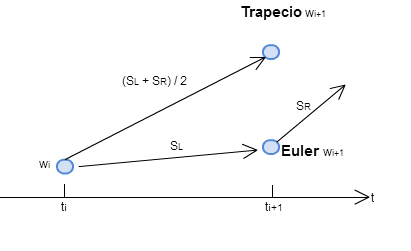
\includegraphics[width=10cm]{./Images/trapecio-vs-euler.png}
			\caption{Esquema visual del método del trapecio explícito.} 
			\label{fig:trapecio-vs-euler}
		\end{figure}

\subsection{Error} \label{sec:trapecio-explicito:error}

\begin{theorem}
El error local del método del trapecio es de orden tres. En consecuencia, el error global del método es de orden dos. 
\end{theorem}
\begin{proof}
Podemos particularizar la expresión del método para $j-1 = 0$ y $j=1$ como 
$y_1=y_0+\frac{h}{2}(f(t_0,y_0)+f(t_0+h,y_0+h K_0)$ siendo $K_0=f(t_0,y_0)$. 

Para obtener el error local suponemos que $y_0$ es exacto, $y_0=y(t_0)$. Claramente, $K_0 = y'(t_0)$. Considerando el desarrollo de Taylor en varias variables para $K_1=f(t_0+h,y_0+h K_0)$ en el punto $(t_0,y_0)$ se tiene:

$K_1 = f(t_0,y_0) + h \frac{\partial f(t_0,y_0)}{\partial t}+h K_0\frac{\partial f(t_0,y_0)}{\partial y}+O(h^{2})=y'(t_0)+hy''(t_0)+O(h^{2})$ 

ya que $\frac{\partial f(t,y(t))}{\partial t} = \frac{\partial f}{\partial t} + y'(t)\frac{\partial f}{\partial y}$

Por lo tanto $y_1=y_0+\frac{h}{2}(2y'(t_0)+hy''(t_0)+O(h^2))=y_0+hy'(t_0)+\frac{1}{2}h^{2}y''(t_0)+O(h^3)$

Por otro lado el desarrollo de $y(t_1)=y(t_0 + h)$ en torno a $t_0$ es 
$y(t_1)=y(t_0)+hy'(t_0)+\frac{1}{2}h^{2}y''(t_0)+O(h^{3})$. 

De donde obtenemos $y(t_1)-y_1=O(h^{3})$ y aplicando el teorema 2.3 sabemos que el error global es $O(h^{2})$.
\end{proof}

Respecto al error de redondeo se tiene que la situación es análoga a la encontrada con las fórmulas de derivación: el error de truncamiento disminuye con h, pero el error de redondeo aumenta, existiendo un valor óptimo para el cual la suma de estos errores es mínima. Este valor óptimo de h suele ser tan pequeño que utilizarlo supone un coste computacional muy grande. 

		\begin{figure}[H]
			\centering
			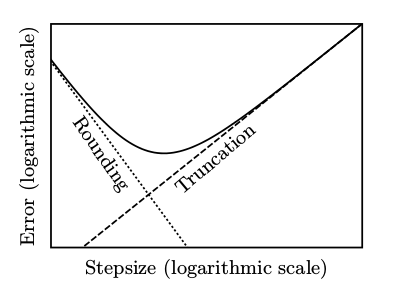
\includegraphics[width=8cm]{./Images/redondeo.png}
			\caption{Combinación de los errores de truncatura y redondeo} 
			\label{fig:redondeo}
		\end{figure}


Así en el caso del método del trapecio, si tomamos $h=\frac{b-a}{N}$ entonces en cada uno de los $N$ pasos se comete un error de redondeo acotado por $\epsilon$ además del error local de truncatura $Ch^{3}$. Globalmente, por lo tanto 
$N(\epsilon+Ch{3})=\frac{\epsilon'}{h}+C'h^{2}$. En una situación ideal la cota $\epsilon$ será del orden de la precisión de la máquina $\mu$ y la constante $C$ será del orden del cubo de la constante de Lipschitz $L^3$ de modo que el valor óptimo para el paso $h$ se obtendría (derivando e igualando a cero) para $h=\frac{\sqrt[3]\mu}{L}$.

Sin embargo, el análisis es bastante más complicado que esto y existen al menos dos vías para su estudio, un modelo más pesimista se pondría en el peor de los casos y un modelo probabilista que se puede encontrar en el libro de Henrici "Discrete Variable Methods in Ordinary Differential Equations". Otros autores como Butcher en su libro "Numerical Methods for Ordinary Differential Equations" en vez de llevar a cabo un análisis detallado de la situación mencionan el uso del llamdo algoritmo de Gill-Moller o "suma compensada". Este algoritmo persigue reducir los efectos de los errores de redondeo.

\subsection{Estabilidad y convergencia} \label{sec:trapecio-explicito:estabilidad}

	Aplicamos este teorema al método del trapecio. En este caso $\phi(t,y,h)=\frac{1}{2}f(t,y)+\frac{1}{2}f(t+h,y+hf(t,y))$. Asumiendo las condiciones que nos dan existencia y unicidad, si f es Lipschitziana en 
	$\{(t,y):a \leq t \leq b, y \in \mathbb{R}\}$ 
	con constante de Lipschitz L entonces:
	
	$|\phi(t,y,h)-\phi(t,y',h)|=|\frac{1}{2}f(t,y)+\frac{1}{2}f(t+h,y+hf(t,y))-\frac{1}{2}f(t,y')-\frac{1}{2}f(t+h,y'+hf(t,y'))| \leq \frac{1}{2}L|y-y'|+\frac{1}{2}L|y+hf(t,y)-y'-hf(t,y')| \leq L |y-y'|+\frac{1}{2}L|hf(t,y)-hf(t,y')|=(L+\frac{1}{2}hL^{2})|y-y'|$ 
	
	Por tanto, $\phi$ satisface una condición de Lipschitz sobre el conjunto 
	$\{(t,y,h):a \leq t \leq b, y \in \mathbb{R}, h \in [0,h_0]\}$ 
	con constante de Lipschizt 
	$L'=L+\frac{1}{2} h_0 L^{2}$ 
	para cualquier $h_0 > 0$. 
	
	Finalmente, si f es continua en 
	$\{(t,y):a \leq t \leq b, y \in \mathbb{R}\}$ 
	entonces $\phi$ es continua en 
	$\{(t,y,h):a \leq t \leq b, y \in \mathbb{R}, h \in [0,h_0]\}$ 
	directamente por la propia definición de $\phi$. 
	
	De este modo podemos aplicar el teorema anterior y tenemos demostrado que el método del trapecio es estable. 
	
	Considerando ahora $\phi(t,y,0)=\frac{1}{2}f(t,y)+\frac{1}{2}f(t,y)=f(t,y)$ tenemos la condición de consistencia expresada anteriormente lo que nos dice que el método es convergente.

%-----------------------------------------------------------------------------------------------------
%	SECCIÓN 3: MÉTODO DEL TRAPECIO ITERATIVO
%-----------------------------------------------------------------------------------------------------

\section{Método del trapecio iterativo} \label{sec:trapecio-iterativo}
	
	 Supóngase que se conoce $y_{i-1}$ para cierto $i \in \{1, 2, \ldots, n\}$ y que, además, se ha obtenido una aproximación inicial para $y_i$. Esta aproximación se denota $w_i^{(0)}$. La expresión (\ref{eq:app}) sugiere evaluar el miembro de la derecha utilizando $w_i^{(0)}$ en lugar de $y_i$ para obtener una nueva aproximación. De esta forma se define
	
	\begin{equation} \label{eq:ti-def}
		w_{i} ^{(j+1)} = y_{i-1} + \frac{h}{2} \left[f(t_{i-1}, y_{i-1}) + f(t_i, w_{i}^{(j)})\right]
	\end{equation}
	
	Nótese que la sucesión definida en (\ref{eq:ti-def}) es esencialmente un método de iteración funcional para obtener un punto fijo de $g(y) = y_{i-1} + \frac{h}{2} \left[f(t_{i-1}, y_{i-1}) + f(t_i, y)\right]$. La primera pregunta que surge es si la sucesión $\{w_{i}^{(j)}\}$ converge. Este hecho se estudia en la Sección \ref{sec:trapecio-iterativo:error}, donde se probará la convergencia bajo determinadas condiciones. En tal caso, se toma $w_i = \lim w_i^{(j)}$ como aproximación de $y_i$. Además, se probará que el error local cometido utilizando esta aproximación es $O(h^3)$.
	
	La segunda cuestión a tratar es cómo aplicar este método para obtener aproximaciones de todos los $t_i$ si solamente se conoce $y_0$. La idea es simple, utilizar la aproximación $w_{i-1}$ como $y_{i-1}$ en la expresión (\ref{eq:ti-def}). De esta forma se obtiene el siguiente método
	
	\begin{equation} \label{eq:ti-def-2}
		\begin{cases}
			w_{i} ^{(j+1)} = w_{i-1} + \frac{h}{2} \left[f(t_{i-1}, w_{i-1}) + f(t_i, w_{i}^{(j)})\right] \\
			w_i = \lim w_{i}^{(j)} \\
		\end{cases}
	\end{equation}

	La aproximación que se toma como $w_i^{(0)}$ suele ser obtenida mediante un método explícito de menor orden, como el método de Euler. Nótese que en tal caso $w_i^{(1)}$ es el resultado de aplicar el método del trapecio explícito partiendo de $w_{i-1}$. Por tanto, el método del trapecio iterativo puede entenderse como una generalización del método del trapecio explícito.
	
	Por otro lado, el método del trapecio iterativo también puede concebirse como un mecanismo para corregir el error cometido por la aproximación inicial. Al método utilizado para calcular la aproximación inicial se le denomina predictor mientras que a la fórmula (\ref{eq:ti-def-2}) se la denomina fórmula correctora. La aplicación de la fórmula correctora al resultado del predictor es lo que se conoce como método predictor-corrector en la literatura especializada.
	
	Por último, en la práctica solo se realizan un número pequeño de iteraciones de la fórmula (\ref{eq:ti-def-2}). Si $j$ es el número de iteraciones escogido, se puede calcular de forma teórica un valor de $j$ de manera que el error $w_i - w_i^{(j)}$ sea tan pequeño como se quiera. En la Sección \ref{eq:ti-def-2} se explica cómo.
	
	
	\subsection{Estudio del error} \label{sec:trapecio-iterativo:error}

		El resultado del estudio de esta cuestión viene dado en la siguiente proposición.
		
		\begin{proposition}
			Si la función $f$ es Lipschitziana en la segunda variable con constante de Lipschitz $L$ y se verifica $\frac{hL}{2} < 1$, entonces la sucesión $\{w_i^{(j)}\}$ converge cuando $j \rightarrow +\infty$. Denotando $w_i = \lim w_i^{(j)}$, se tiene además $\left|y_{i} - w_{i}\right| = O(h^3)$.
		\end{proposition}
		
		\begin{proof}
			La prueba se centra en comprobar que $\{w_i^{(j)}\}$ es una sucesión de Cauchy. En primer lugar, se estudia $\{w_{i}^{(j+1)} - w_{i}^{(j)}\}$. Utilizando la condición de Lipschitz
			
			\begin{equation*}
			\left|w_{i}^{(j+1)} - w_{i}^{(j)}\right| \le \frac{h}{2} \left| f(t_i, w_i^{(j)}) - f(t_i, w_i^{(j-1)}) \right| \le \frac{hL}{2} \left| w_i^{(j)} - w_i^{(j-1)} \right| \le \ldots \le \left(\frac{hL}{2}\right)^j \left|w_i^{(1)} - w_i^{(0)}\right|
			\end{equation*}
			
			Posteriormente se utiliza la desigualdad obtenida para conseguir acotar $\left|w_{i}^{(j+q)} - w_{i}^{(j)}\right|$. 
			
			\begin{equation*}
			\left|w_{i}^{(j+q)} - w_{i}^{(j)}\right| \le \sum_{k = j} ^ {j+q} \left|w_i^{(k)} - w_i^{(k-1)}\right| \le \sum_{k = j} ^ {j+q} \left(\frac{hL}{2}\right)^{k-1} \left|w_i^{(1)} - w_i^{(0)}\right| = \left|w_i^{(1)} - w_i^{(0)}\right| \sum_{k = j} ^ {j+q} \left(\frac{hL}{2}\right)^{k-1}
			\end{equation*}
			
			Como $\frac{hL}{2} < 1$, se tiene que la serie $\sum_{j \ge 0} \left(\frac{hL}{2}\right) ^j$ converge. Por consiguiente, es de Cauchy. Aplicando este hecho en la expresión previa se obtiene que $\{w_i^{(j)}\}$ es una sucesión de Cauchy. 
			
			Nótese que tomando límites en (\ref{eq:ti-def}) se obtiene la siguiente igualdad
			
			\begin{equation} \label{eq:prop2.2}
			w_{i} = y_{i-1} + \frac{h}{2} \left[f(t_{i-1}, y_{i-1}) + f(t_i, w_{i})\right]
			\end{equation}
			
			
			Por último, se estudia $\left|y_{i} - w_{i}\right|$. Restando las expresiones (\ref{eq:trapecio-igualdad}) y (\ref{eq:prop2.2}) se obtiene
			
			$$ \left|y_{i} - w_{i}\right| = \left|\frac{h}{2} \left[f(t_{i},y_{i}) - f(t_{i}, w_{i})\right] - \frac{h^3}{12}y^{3)}(\xi)\right| \le \frac{h}{2} \left|f(t_{i},y_{i}) - f(t_{i}, w_{i})\right| + \frac{h^3}{12}\left|y^{3)}(\xi)\right| \le$$
			$$ \frac{hL}{2} \left|y_{i} - w_{i}\right| + \frac{h^3}{12}\left|y^{3)}(\xi)\right| $$
			
			Por tanto, agrupando los $\left|y_{i} - w_{i}\right|$ se tiene la siguiente desigualdad
			
			\begin{equation*}
			\left|y_{i} - w_{i}\right| \le \frac{2}{2 - HL}\frac{h^3}{12}\left|y^{3)}(\xi)\right| = O(h^3)		
			\end{equation*}
			
		\end{proof}


%-----------------------------------------------------------------------------------------------------
%	SECCIÓN X: ARTÍCULO
%-----------------------------------------------------------------------------------------------------

\section{Artículo de investigación} \label{sec:paper}

\section{Ejercicios teórico-practicos}

Ejercicio 2: dada la ecuación $y'=t+y^2$ con $y(1)=1$ aproximar mediante el método del trapecio: a) y(1,2) con 2 pasos (h=0,1) y b) y(1,2) con 4 pasos (h=0,05). Si el error global es de la forma $Ch^2$, estimar el valor de C apartir de los resultados anteriores. Determinar h para que el error sea del orden de $10^{-4}$.

Solución:

    \begin{table}[H]
		\centering
		\begin{tabular}{|| c | c | c | c | c ||}
			\hline
			\hline $j$ &  $t_{j-1}$ & $y_{j-1}$ & $t_j$ & $y_j$ \\
			\hline 1 & 1.00 & 2.000000 & 1.10 & 2.617500 \\
			\hline 2 & 1.10 & 2.617500 & 1.20 & 3.657368 \\
		\end{tabular}
		\caption{Trapecio con $h=0.1$}
		\label{table:trapecio-ej2}
	\end{table}
	
	 \begin{table}[H]
		\centering
		\begin{tabular}{|| c | c | c | c | c ||}
			\hline
			\hline $j$ &  $t_{j-1}$ & $y_{j-1}$ & $t_j$ & $y_j$ \\
			\hline 1 & 1.00 & 2.000000 & 1.05 & 2.277813 \\
			\hline 2 & 1.05 & 2.277813 & 1.10 & 2.628941 \\
			\hline 3 & 1.10 & 2.628941 & 1.15 & 3.087423 \\
			\hline 4 & 1.15 & 3.087423 & 1.20 & 3.712364 \\
		\end{tabular}
		\caption{Trapecio con $h=0.05$}
		\label{table:trapecio-ej2.1}
	\end{table}
	
	Gracias a estos cálculos y como en el enunciado se nos dice que el error global es de la forma $Ch^2$ (lo que es coherente con el error global del método explícito) podemos escribir:
	
	$y(1.2) - 3.657368 = C(0.1)^2$
	$y(1.2) - 3.712364 = C(0.05)^2$
si restamos ambas ecuaciones y despejamos se obtiene:
	$C=7.33$
	Asumiendo entonces que el error global puede representarse mediante $7.33 h^2$ para que sea de orden $10^{-4}$ debe ser $h=3.7$ $10^{-3}$


%-----------------------------------------------------------------------------------------------------
%	SECCIÓN X: CONCLUSIÓN
%-----------------------------------------------------------------------------------------------------


\section{Conclusión} \label{sec:conclusion}


%-----------------------------------------------------------------------------------------------------
%	SECCIÓN X: REFERENCIAS
%-----------------------------------------------------------------------------------------------------

\printbibliography


\end{document}
